\section{Installation instructions}

LANS is a Matlab-based program. Thus, a core \textbf{Matlab} installation, along with image processing and statistical toolboxes, is required to run LANS and perform basic functions. This makes it possible to run LANS on a variety of operating systems, including Linux, Microsoft Windows and MacOS. However, this also limits LANS to users with access to a Matlab license. Additional functionality of LANS is achieved by integrating the program with \textbf{\LaTeX} (for exporting results in a nicely formatted PDF output) and data compression programs such as \textbf{zip} (for decompressing input files and compressing output generated by LANS), both of which are available for free.

%%

\subsection{Install Matlab}
\setcounter{step}{0}

\goldbox{}
Matlab is available from \url{www.mathworks.com} and requires a license. It is useful to check whether your institution has a site-license (e.g., your university may have one for all students and academic staff). 
\tcbe

\sbx{Install the \ttt{core Matlab} and two toolboxes: \ttt{image processing toolbox} and \ttt{statistics and machine learning toolbox}. }

\nbx{Version 2019b of Matlab is most recommended to ensure that all features of LANS work as designed. LANS works with newer Matlab versions as well, however, there is a risk that some functionality will issue errors due to less than perfect back-compatibility of Matlab.}

\nnb{Some output generated by LANS, e.g., information generated during the alignment of planes and stored in the file \ttt{xyalign.mat}, may not be loaded correctly by an older Matlab version if it was generated by a~newer Matlab version. Thus, if you plan to use LANS in collaboration with other people, e.g., by sharing the files generated by LANS among each other, it is recommended that everyone in the team uses the same Matlab version.}

%%

\subsection{Install \LaTeX}
\setcounter{step}{0}

\goldbox{}
\LaTeX\ is required to enable export of graphical output as tagged PDF documents. 
\tcbe

\sbx{To install \LaTeX, use one of the well-established \LaTeX\ distributions for your operating system, as described on the \href{https://www.latex-project.org/get/}{\LaTeX\ project} website (e.g., \ttt{texlive} for Linux, \ttt{MikTeX} for Windows, \ttt{MacTex} for MacOS). Note that the on-line LaTeX service, such as Overleaf, is insufficient; you really need a locally installed \LaTeX\ distribution.}
 
\sbx{To correctly integrate \LaTeX\ with LANS, check that the following executables and packages are installed and working:
 
\begin{itemize}
\item[--] executables: \ttt{epstopdf}, \ttt{pdflatex}
\item[--] packages: \ttt{graphicx}, \ttt{geometry}, \ttt{url}, \ttt{hyperref}, \ttt{adjustbox}
\end{itemize}}
 
\nbx{If you have never used \LaTeX\ on your computer, it may be that some \LaTeX\ packages, parti\-cu\-larly \ttt{geometry}, \ttt{hyperref} and \ttt{adjustbox}, are not installed during the `standard' installation steps. As a result, the execution of the LANS functions \lans{Export LaTeX and PDF output} (main LANS window) or \lans{Export images for each variable as PDF} (Process metafile window) may get stuck if the packages are missing. }

\nnb{If this happens and you are working under Microsoft Windows, you can fix this problem by compiling the \ttt{tex} file using the native \LaTeX\ environment (e.g., open the \ttt{tex} file in the default editor of your \LaTeX\ distribution and then compile it into a \ttt{pdf} output from there). When doing so, the missing \LaTeX\ packages should automatically be installed and the \ttt{tex} file should compile into a~correct \ttt{pdf} output. Once this is done, the automatic \LaTeX\ compilation from within Matlab will also work.}

\nnb{If you are using Linux or MacOS, you need to do a~little bit of internet searching to figure out how to ensure that all the required \LaTeX\ packages are installed.}

%%

\subsection{Install software for compressing/decompressing files}
\setcounter{step}{0}

\goldbox{}
This software is required for two main reasons:

\begin{enumerate}
 
\item It enables you to load compressed nanoSIMS datasets (\ttt{im.zip} files) by LANS. This is a~useful feature because \ttt{im.zip} files have roughly 5--10-fold smaller size than the original \ttt{im} files generated by the Cameca's nanoSIMS measurement software. It is recommended to store and distribute the raw data files by first compressing them with the \ttt{zip} program (extension \ttt{im.zip}). 

\item It allows you to compress the processed data generated by LANS. This is convenient for making data backups, since it is much more efficient to upload and download few compressed folders than hundreds of smaller files present in those folders.

\end{enumerate}
\tcbe

\sbx{If you work under Microsoft Windows, it is recommended to install \ttt{7-Zip} (freeware). If you work under Linux and MacOS systems, you do not need to do anything because \ttt{zip} and \ttt{unzip} are available by default.}

%%

\subsection{Install Look@NanoSIMS}
\setcounter{step}{0}

\goldbox{}
LANS is installed by simply copying the source files (\ttt{m} and \ttt{fig}) to a~folder on your computer.
\tcbe

\sbx{For convenience, the compressed file containing the \emph{latest version of LANS} is stored in this \href{https://www.dropbox.com/sh/gyss2uvv5ggu2vl/AABViAmt9WHryEP_xZBrCG_La?dl=0}{Dropbox folder}. Click on the \ttt{program} folder and then download the file \ttt{LANS-latest-src.zip}.}

\sbx{Unzip \ttt{LANS-latest-src.zip} to a folder of your choice.}

\sbx{Rename the \ttt{src} folder using a more reasonable name (e.g., \ttt{LANS-2025-07-27}, where the date refers to the LANS version).}

\nbx{In case the Dropbox link above does not work, because it became outdated or the official distribution location changed, visit the LANS github repository or try to search the internet for more updated information. For users familiar with git and github, LANS can be downloaded by pulling the source code from the \ttt{src} folder in the LANS github repository: \url{https://github.com/lpolerecky/LANS}.}

%%

\subsection{Starting LANS for the first time}
\setcounter{step}{0}

Before you run LANS for the first time, read through the content of the files \ttt{lookatnanosims.m} and \ttt{lans\_paths.m}, which can be found in the same location where you installed LANS. These two files contain important settings you need to adjust to reflect your specific local installation of LANS. For example, you can specify there:
%\setlist{nolistsep}

\begin{itemize}%[noitemsep]
\item[--] locations of the compression/decompression software,
\item[--] location of the PDF viewer,
\item[--] default name of the file containing regions of interest (ROIs),
\item[--] default extension of the raw data files.
\end{itemize}

\nbx{If you browse through the LANS installation files, you will notice that the \ttt{*.fig} files, which define the graphical user interface (GUI), appear in two sub-folders: \ttt{figs} and \ttt{figs\_win}. This is required because GUI defined on Unix-like and Windows platforms do not look the same. This is an issue due to --- apparently --- limited cross-platform compatibility of Matlab visual objects. However, this issue is not important for you as an end-user of LANS. You only need to be aware of it. Should you wish to modify any of the \ttt{*.fig} files, you will need to modify those that correspond to your operating system.}

%%

\subsection{Starting LANS on a regular basis}
\setcounter{step}{0}

\sbx{Start Matlab.}

\sbx{Set the current folder to the folder where you installed LANS. You can do this through the menu or, more easily, entering one of the following commands in the Matlab console. The precise syntax depends on whether you use Windows, Linux or MacOS, and on the path where you installed LANS. Thus, you will need to adapt it according to your local settings.

\ttt{cd c:$\backslash$programs$\backslash$LANS}

\ttt{cd /home/your\_username/programs/LANS}}

\sbx{Once you are in the correct folder, enter the following command in the Matlab console:

\ttt{lookatnanosims}}

\begin{figure}[!t]
\centering
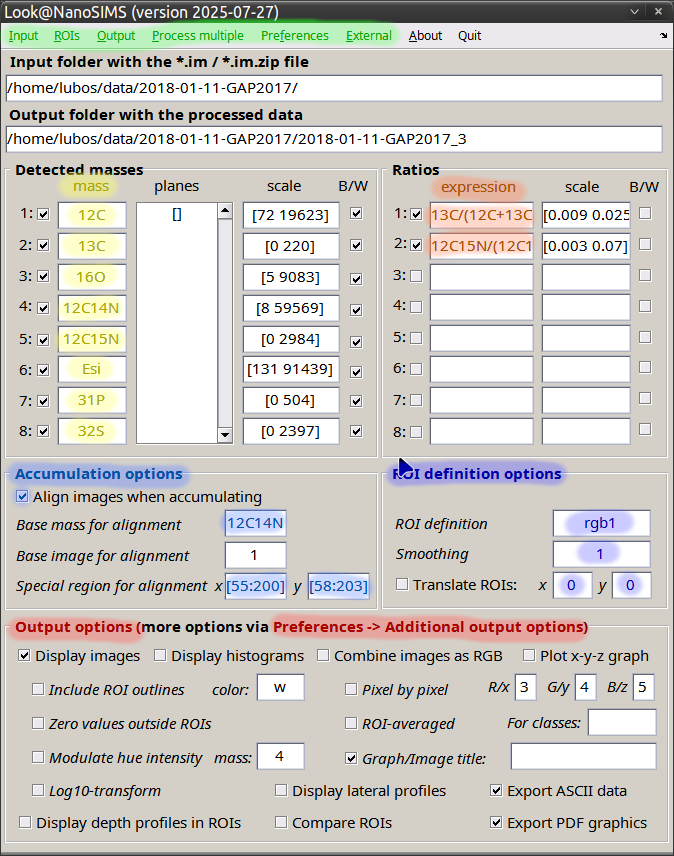
\includegraphics[scale=0.5]{figs1/LANS-maingui}
\caption{\label{fig1:mainLANSgui}%
Main window of the Look@NanoSIMS program.}
\end{figure}

\nbx{If everything is set up correctly, the main LANS graphical user interface (GUI) will open, as shown in Fig.~\ref{fig1:mainLANSgui}. You can start from there, as described in the following sections of this document.}

\nnb{During the data processing session, LANS provides quite a lot of useful information in the Matlab console. Thus, it is a good idea to \emph{always} keep an eye on the output in the console. You can do this by arranging your desktop such that both the LANS and Matlab console windows are visible at the same time. This is also useful in case you encounter an error while working in LANS. These errors will be shown in the console, too.}

%%

\subsection{Updating LANS}
\setcounter{step}{0}

\s LANS is updated quite regularly. You can update it easily by entering in the Matlab console:

\ttt{lans\_webupdate} 

\bul You need to be in the folder where LANS is installed to run this command. In the process, you will be prompted to make a backup of your older LANS version, which is recommended to do, just in case.

\bul If you are familiar with \ttt{git}, you can update LANS by pulling the latest sources from the LANS github repository \url{https://github.com/lpolerecky/LANS}.
